\usetikzlibrary{arrows.meta}
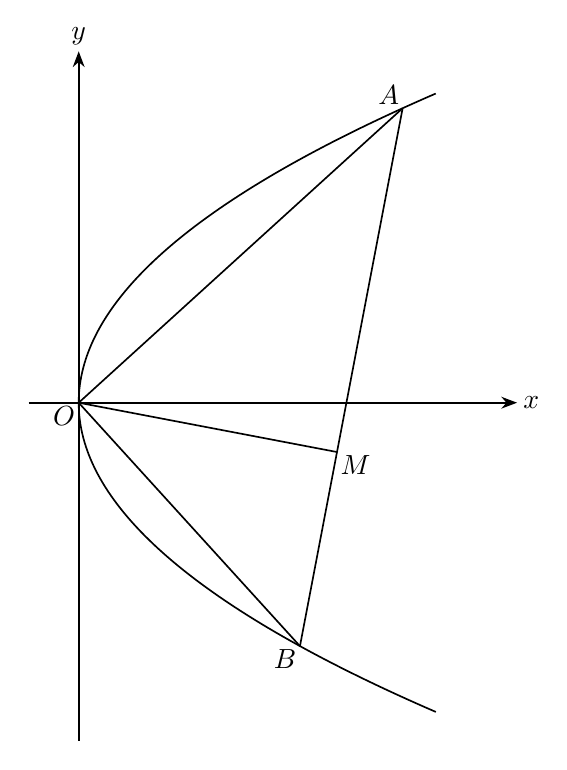
\begin{tikzpicture}[x=0.85cm,y=0.85cm,line width=.6pt,font=\normalsize,>=Stealth]
\coordinate (O) at (0,0);
\coordinate (A) at (4.84,4.4);
\coordinate (B) at (3.30578512,-3.63636364);
\coordinate (M) at (3.85934198,-0.73678303);
\draw[->] (-0.75,0)--(6.55,0) node[right,inner sep=0pt,xshift=2pt] {$x$};
\draw[->] (0,-5.05)--(0,5.25) node[above,inner sep=0pt,yshift=2pt] {$y$};
\draw[domain=-4.62:4.62,samples=141] plot ({0.25*\x*\x},{\x});
\draw (O)--(A);
\draw (O)--(B);
\draw (A)--(B);
\draw (O)--(M);
\node[below left,inner sep=1pt] at (O) {$O$};
\node[above left,inner sep=1pt] at (A) {$A$};
\node[below left,inner sep=1pt] at (B) {$B$};
\node[below right,inner sep=1pt] at (M) {$M$};
\end{tikzpicture}
